%XXX-Peter: Does this subsection really belong here? My understanding is that it describes
%the full picture (Sections 4 and 5) and not just what is happening in this section.
% \subsection{Structure of our proof}
% \label{subsec:proof-structure}
%
% % XXX-Peter: This whole paragraph can go away; we already said this before.
% In order to prove the correctness of X25519 in TweetNaCl code \TNaCle{crypto_scalarmult},
% we use VST to prove that the code matches our functional Coq specification of \Coqe{RFC}.
% Then, we prove that our specification of the scalar multiplication matches the mathematical definition
% of elliptic curves and Theorem 2.1 by Bernstein~\cite{Ber06} (\sref{sec:maths}).
%
% Verifying \TNaCle{crypto_scalarmult} also implies verifying all the functions
% subsequently called: \TNaCle{unpack25519}; \TNaCle{A}; \TNaCle{Z}; \TNaCle{M};
% \TNaCle{S}; \TNaCle{car25519}; \TNaCle{inv25519}; \TNaCle{set25519}; \TNaCle{sel25519};
% \TNaCle{pack25519}.
%
% We prove that the implementation of X25519 is \textbf{sound}, \ie:
% \begin{itemize}
% \item absence of access out-of-bounds of arrays (memory safety).
% \item absence of overflows/underflow in the arithmetic.
% \end{itemize}
% We also prove that TweetNaCl's code is \textbf{correct}:
% \begin{itemize}
% \item X25519 is correctly implemented (we get what we expect) .
% \item Operations on \TNaCle{gf} (\TNaCle{A}, \TNaCle{Z}, \TNaCle{M}, \TNaCle{S})
% are equivalent to operations ($+,-,\times,x^2$) in $\Zfield$.
% \item The Montgomery ladder computes the multiple of a point.
%   %XXX-Peter: We don't prove this last statement in this section
% \end{itemize}
%
% In order to prove the soundness and correctness of \TNaCle{crypto_scalarmult},
% we reuse the generic Montgomery ladder defined in \sref{sec:Coq-RFC}.
%
% We define a high-level specification by instantiating the ladder with a generic
% field $\K$, this allows us to prove the correctness of the ladder with respect
% to the theory of elliptic curves.
% This high-level specification does not rely on the parameters of Curve25519.
% We later specialize $\K$ with $\Ffield$, and the parameters of Curve25519 ($a = 486662, b = 1$),
% to derive the correctness of \coqe{RFC} (\sref{sec:maths}).
% %XXX-Peter: not in this section, correct?
%
% We define a mid-level specification by instantiating the ladder over $\Zfield$.
% Additionally we also provide a low-level specification close to the \texttt{C} code
% (over lists of $\Z$). We show this specification to be equivalent to the
% \emph{semantic version} of C (Clight) using VST.
% This low level specification gives us the soundness assurance.
%
% RFC~7748's X25519 formalization (\sref{sec:Coq-RFC}) takes as input list of $\Z$.
% However the inner Montgomery ladder operates on $\Zfield$. We show its equivalence
% with our mid-level and low-level specifications.
%
% By showing that operations over instances ($\K = \Ffield$, $\Zfield$, list of $\Z$) are
% equivalent, we bridge the gap between the different level of specification
% with Curve25519 parameters.
% As such, we prove all specifications to equivalent (\fref{tikz:ProofStructure}).
% This guarantees us the correctness of the implementation.
%
% \begin{figure}[h]
%   \centering
%   \begin{tikzpicture}[textstyle/.style={black, anchor= south west, align=center}]

    \filldraw[draw=orange!10!doc@lstbackground, fill=doc@lstbackground, thick] (0.25,0.5) rectangle (4.5,5.5);
    % node[textstyle, anchor=west, draw=yellow, fill=yellow!20, thick, minimum width=5.5cm,minimum height=5cm] {};

    \draw (4.5,5.5)  node[anchor=north east, inner sep=0pt] (russell) {
\includegraphics[width=.03\textwidth]{img/coq_logo.png}};

    \draw (0.5,-1) node [textstyle, anchor=west, draw=black, thick, minimum width=3cm,minimum height=0.5cm] (longlong) {\texttt{long long[16]}};
    \draw (0,-1) node [anchor=east] (longlongdef) {\texttt{C} code};
    \draw (2.25,-0.1) node [anchor=west] (app) {\texttt{clightgen}};


    \draw (0.5,1) node [textstyle, anchor=west, draw=black, thick, minimum width=3cm,minimum height=0.5cm] (clight) {\texttt{tptr tlong}};
    \draw (0,1) node [anchor=east] (clightdef) {Clight};

    \draw [thick, ->] (longlong.north) -- (clight.south);

    \begin{scope}[yshift=1 cm,xshift=0 cm]

      \draw (0.5,2) node [textstyle, anchor=west, draw=black, thick, minimum width=3cm,minimum height=0.5cm] (ll) {\texttt{list} $\Z$};
      \draw (0,2) node [anchor=east] (shn) {Low Level};

      \draw [thick,double, <->, >=implies] (clight.north) -- (ll.south);
      \draw (2.25,1) node[anchor=west, inner sep=0pt] (chain) {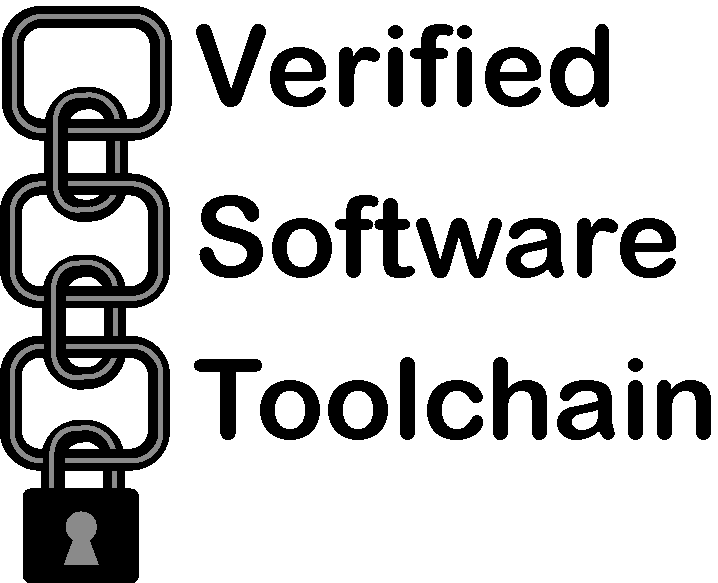
\includegraphics[width=.07\textwidth]{img/chain.png}};


      \draw (0.5,3) node [textstyle, anchor=west, draw=black, thick, minimum width=3cm,minimum height=0.5cm] (ml) {$\Zfield$};
      \draw (0,3) node [anchor=east] (shn) {Mid Level};

      \draw[thick,double, <->, >=implies] (ll.north) -- (ml.south);

      \draw (0.5,4) node [textstyle, anchor=west, draw=black, thick, minimum width=3cm,minimum height=0.5cm] (hl) {$\K$};
      \draw (0,4) node [anchor=east] (shn) {High Level};

      \draw[thick,double, <-, >=implies] (ml.north) -- (hl.south);
    \end{scope}
\end{tikzpicture}

%   \caption{Structural construction of the proof}
%   \label{tikz:ProofStructure}
% \end{figure}
